\documentclass[12pt, titlepage]{article}

\usepackage{booktabs}\usepackage{fullpage}
\usepackage[round]{natbib}
\usepackage{multirow}
\usepackage{booktabs}
\usepackage{tabularx}
\usepackage{graphicx}
\usepackage{float}
\usepackage{hyperref}
\usepackage{pdfpages}
\hypersetup{
    colorlinks,
    citecolor=black,
    filecolor=black,
    linkcolor=red,
    urlcolor=blue
}
\usepackage[round]{natbib}

\title{SE 3XA3: Test Plan\\Snake 2.0}

\author{Team \#34, Team Send Help
		\\ Harrison Lau	(lauh3)
		\\ Geroge Mo	(moz)
		\\ Vanessa Truong	(truonv1)
}

\date{\today}


\begin{document}

\maketitle

\pagenumbering{roman}
\tableofcontents
\listoftables
\listoffigures

\begin{table}[bp]
\caption{\bf Revision History}
\begin{tabularx}{\textwidth}{p{3cm}p{2cm}X}
\toprule {\bf Date} & {\bf Version} & {\bf Notes}\\
\midrule
Oct 26, 2017 & 1.0 & Created Document and finished Section 1\\
Oct 27 & 1.1 & Finished Section 2, 3\\
Oct 27 & 1.2 & Finished Sections 2.5, 3.3, 5, 7\\
Dec 4 & 2.0 & Updated manual and unit testing details\\
\bottomrule
\end{tabularx}
\end{table}

\newpage

\pagenumbering{arabic}

This document contains all information regarding the testing plans for for Snake 2.0. It will be used for future reference and will be updated accordingly if any test plans are altered or added.

\section{General Information}

\subsection{Purpose}
The purpose of our project is to reimplement the classic 2D arcade game, Snake, retitled to Snake 2.0, and enhance it with additional features such as power-ups, obstacles, and changeable map shapes. A part of this goal is to discover all potential errors and bugs that may occur in our implementation. Hence, this document will outline our plans for testing our program to verify and validate that it meets all requirements presented in our SRS document, and the approaches that we will take to pinpoint the errors in our program.

\subsection{Scope}
The scope of our testing will cover all basic functionalities of the original version of Snake integrated with the functionalities of our added features. It will also cover memory storage, specifically whether the scoreboard properly updates. Snake 2.0 is an interactive game, and thus, there will also be testing conducted on input and output responses, particularly with regards to the menu functions and whether the gameplay keys correctly correspond with their intended functionalities. A general outline of what features will be tested is here:
\begin{enumerate}
\item Power-ups:
\begin{itemize}
\item Speed Increase
\item Speed Decrease
\item Self-collision invincibility
\end{itemize}
\item In-Game I/O Responses
\begin{itemize}
\item Properly responds to up, down, left, right keys
\item Map Size Changes (whether the selected map size has been activated)
\end{itemize}
\item Menu I/O Responses (Button clicks redirect user to corresponding page)
\item Memory Storage (Scoreboard properly updates)
\item Performance (How timely I/O responses are, points counter accuracy)
\end{enumerate}

\subsection{Acronyms, Abbreviations, and Symbols}
	
\begin{table}[hbp]
\caption{\textbf{Table of Abbreviations}} \label{Table}

\begin{tabularx}{\textwidth}{p{3cm}X}
\toprule
\textbf{Abbreviation} & \textbf{Definition} \\
\midrule
SRS & Software Requirements Specifications document\\
\bottomrule
\end{tabularx}

\end{table}

\begin{table}[!htbp]
\caption{\textbf{Table of Definitions}} \label{Table}

\begin{tabularx}{\textwidth}{p{3cm}X}
\toprule
\textbf{Term} & \textbf{Definition}\\
\midrule
Snake 2.0 & Our reimplementation/redevelopment/program  name\\
Snake & Refers to in-game snake\\
pellet & Refers to what the Snake eats. Triggers its growth, power-ups and obstacles\\
boundary & Refers to the walls of the in-game map\\
\bottomrule
\end{tabularx}

\end{table}	

\subsection{Overview of Document}
The test plan document outlines in detail how Snake 2.0 will undergo the software testing process. It will describe in-depth how all features of Snake 2.0 will be tested, backed up with the testing procedures that will be used for each feature.
 
\section{Plan} 	
\subsection{Software Description}
Snake 2.0 is a reimplementation of the original Snake game. The open-source code is done in JavaScript. For the purposes and scope of our project, Snake2.0 will be programmed in Java. Ideally, the finished code will follow the Model-View-Controller pattern, where the Model will manage the application data, the View will be responsible for the game display, and the Controller will process input and output commands. The GUI components from the Swing and Abstract Window Toolkit package will heavily be used for buiding the Snake 2.0 GUI. 

\subsection{Test Team}
The test team consists of the following project members:
\begin{itemize}
\item Harrison Lau
\item George Mo
\item Vanessa Truong
\end{itemize}
The test team will be responsible for carrying out and executing test procedures, debugging all detected errors from the running test cases, and ensuring the finished program passes all test cases. The test cases will be divided evenly amongst all team members.

\subsection{Automated Testing Approach}
As Snake 2.0 has a number of additional features as mentioned above, testing procedures have been written for several of them. However, automated testing will exclude some of Snake 2.0's functions, such as the menu GUI, as it will prove to be more time consuming than beneficial. The GUI aspects and all functions of the application that require mouse and keyboard inputs will be tested manually. More so, for every implemented feature that is integrated with the game, testing will need to be conducted for that feature independently, and then in coexistence with the other features. This is to ensure that: 1) The feature has been implemented properly, and 2) The feature has been properly implemented for synchronization with all other in-game elements. There are also many additional components in the game menu that will affect the in-game functionality, such as the map-changing option, which will require manual or autoated testing.

With that being said, automated testing will be performed after every implemented feature on its individual correctness (unit testing) and then on the system's correctness with the added feature (integration testing). There will be automated tests conducted on the in-game functionality (points counter, number of dots on the Snake, pellet growth and activation, etc.), aiding our regression testing. This will maximize the efficiency of our test process since Snake 2.0 will incorporate many new major elements and minor components, and manually testing certain aspects of the game's functionality after each one will become repetititve. Manual testing will be necessary to test certain features that will be less feasible to test through automatation. In most cases, testing will fall under functional (or black box) testing to uncover possible bugs in the game's functionality.

Automation tests will be reviewed and maintained after a new feature, which will undergo automated testing, is added. However, for every newly designed test, manual testing will be conducted at least once before automating it.

\subsection{Testing Tools}
The JUnit testing framework will be used for automating the unit tests and integration tests for several of the in-game functionalities for Snake 2.0.

\subsection{Testing Schedule}
		
See Gantt Chart \hyperref[gantt]{here}.

\section{System Test Description}
\label{se:STD}
	
\subsection{Tests for Functional Requirements}
Note that the 'Outputs' for all tests described refer to the expected outputs of our program, as these tests have not been performed yet. 

\subsubsection{Menu GUI}

\begin{enumerate}

\item{FR-P-1\\}
\label{fr:p-1}

Type: Functional, Dynamic, Manual
					
Initial State: Start-up menu of Snake 2.0
					
Input: User selects 'Play' button
					
Output: In-game mode is activated
					
How test will be performed: Snake 2.0 will be opened to the start-up menu window. The 'Play' button will be selected to check whether it activates in-game mode, if it redirects to another page, or if there are any errors.   
			
\paragraph{How to Play}
		
\item{FR-HTP-1\\}
\label{fr:htp-1}

Type: Functional, Dynamic, Manual
					
Initial State: Start-up menu of Snake 2.0
					
Input: User selects 'How to Play' button
					
Output: User is redirected to 'How to Play' page
					
How test will be performed: Snake 2.0 will be opened to the start-up menu window. The 'How to Play' button will be selected to check whether it redirects to the page containing information on how to play, if it redirects to another page, or if there are any errors.   

\item{FR-HTP-2}
\label{fr:htp-2}

Type: Functional, Dynamic, Manual

Initial State: 'How to Play' page 

Input: User selects the 'Back' button

Output: User is redirected to the start-up menu

How test will be performed: Snake 2.0 will be opened to the start-up menu, and then 'How to Play' will be selected. The 'Back' button will then be selected to check whether it redirects to the start-up menu, if it redirects to another page, or if there are any errors.   

\item{FR-HTP-3}
\label{fr:htp-3}

Type: Functional, Dynamic, Manual

Initial State: 'How to Play' page 

Input: User selects the 'Play' button

Output: In-game mode is activated

How test will be performed: Snake 2.0 will be opened to the start-up menu, and then 'How to Play' will be selected. The 'Play' button will then be selected to check whether in-game mode is activated from the 'How to Play' page, if it redirects to another page, or if there are any errors.   

\paragraph{Change Map}

\item{FR-CM-1}
\label{fr:cm-1}

Type: Functional, Dynamic, Manual

Initial State: Start-up menu of Snake 2.0 

Input: User selects the 'Change Map' button

Output: User is redirected to the 'Change Map' page

How test will be performed: Snake 2.0 will be opened to the start-up menu, and then 'Change Map' will be selected to check whether it redirects to the page with different map selections, if it redirects to another page, or if there are any errors.   

\item{FR-CM-2}
\label{fr:cm-2}

Type: Functional, Dynamic, Manual

Initial State: 'Change Map' page

Input: User selects the 'Back' button

Output: User is redirected to the start-up menu

How test will be performed: Snake 2.0 will be opened to the start-up menu, and then 'Change Map' will be selected. The 'Back' button will then be selected to check whether it redirects to the start-up menu, if it redirects to another page, or if there are any errors.   

\item{FR-CM-3}
\label{fr:cm-3}

Type: Functional, Dynamic, Manual

Initial State: 'Change Map' page

Input: User selects Map 1

Output: Map 1 is activated and application transitions to in-game mode

How test will be performed: Snake 2.0 will be opened to the start-up menu, and then 'Change Map' will be selected. Map 1 will then be selected and application will activate in-game mode to check if Map 1 has been applied.

\item{FR-CM-4}
\label{fr:cm-4}

Type: Functional, Dynamic, Manual

Initial State: 'Change Map' page

Input: User selects Map 2

Output: Map 2 is activated and application transitions to in-game mode

How test will be performed: Snake 2.0 will be opened to the start-up menu, and then 'Change Map' will be selected. Map 2 will then be selected and application will activate in-game mode to check if Map 2 has been applied.

\item{FR-CM-5}
\label{fr:cm-5}

Type: Functional, Dynamic, Manual

Initial State: 'Change Map' page

Input: User selects Map 3

Output: Map 3 is activated and application transitions to in-game mode

How test will be performed: Snake 2.0 will be opened to the start-up menu, and then 'Change Map' will be selected. Map 3 will then be selected and application will activate in-game mode to check if Map 3 has been applied.

\subsubsection{In-Game Score Counter}

\item{FR-SCRCTR-1}
\label{fr:scrctr-1}

Type: Functional, Dynamic, Unit, Manual

Initial State: In-game mode

Input: No initial input

Output: Snake's score is 100 by default

How test will be performed: Snake 2.0 will be in in-game mode and the score counter will be checked to ensure that it is at 100.

\item{FR-SCRCTR-2}
\label{fr:scrctr-2}

Type: Functional, Dynamic, Unit, Manual

Initial State: In-game mode

Input: Snake will move 7 times

Output: Snake's score will decrement by 1 from 100, resulting with 99

How test will be performed: Snake 2.0 will be in in-game mode and make at least 7 moves, and the score counter will be checked to ensure it is 99.

\item{FR-SCRCTR-3}
\label{fr:scrctr-3}

Type: Functional, Dynamic, Unit, Manual

Initial State: In-game mode

Input: Snake eats a pellet

Output: Snake's score is incremented by 10 from the default score

How test will be performed: Snake 2.0 will be in in-game mode and will consume a pellet. The score counter will be checked to see if it has been incremented by 10.

\subsubsection{In-Game Power-ups}

\item{FR-SPD-1}
\label{fr:spd-1}

Type: Functional, Dynamic, Manual

Initial State: In-game mode

Input: Snake eats 'Speed-up' pellet

Output: Snake's speed is increased

How test will be performed: Snake 2.0 will be in in-game mode, and we will continously move the Snake to eat pellets in the map until a 'Speed-up' pellet is eaten to check if Snake's speed has  been increased.

\item{FR-SPD-2}
\label{fr:spd-2}

Type: Functional, Dynamic, Manual

Initial State: In-game mode

Input: Snake eats pellets

Output: 'Speed-up' pellets randomly spawn

How test will be performed: Snake 2.0 will be in in-game mode, and we will continously move the Snake to eat pellets in the map until a 'Speed-up' pellet is eaten. The number of pellets eaten inbetween each 'Speed-up' pellet that spawns will be counted to check that spawning is random.

\item{FR-SPD-3}
\label{fr:spd-3}

Type: Functional, Dynamic, Manual

Initial State: In-game mode

Input: Snake eats 'Slow-down' pellet

Output: Snake's speed is decreased

How test will be performed: Snake 2.0 will be in in-game mode, and we will continously move the Snake to eat pellets in the map until a 'Slow-down' pellet is eaten to check if Snake's speed has  been decreased.

\item{FR-SPD-4}
\label{fr:spd-4}

Type: Functional, Dynamic, Manual

Initial State: In-game mode

Input: Snake eats pellets

Output: 'Slow-down' pellets randomly spawn

How test will be performed: Snake 2.0 will be in in-game mode, and we will continously move the Snake to eat pellets in the map until a 'Slow-down' pellet is eaten. The number of pellets eaten inbetween each 'Slow-down' pellet that spawns will be counted to check that spawning is random.

\item{FR-SPD-5}
\label{fr:spd-5}

Type: Functional, Dynamic, Unit, Manual

Initial State: In-game mode

Input: Snake eats 'Speed-up' pellet

Output: Snake has speed-up power-up for 35 step counts

How test will be performed: Snake 2.0 will be in in-game mode, and we will continously move the Snake to eat pellets in the map until a 'Speed-up'  pellet is eaten. The state for an active speed-up pellet will be checked to see if true and the step count variable will be checked for incrementation. 

\item{FR-SPD-6}
\label{fr:spd-6}

Type: Functional, Dynamic, Unit, Manual

Initial State: In-game mode

Input: Snake eats 'Slow-down' pellet

Output: Snake has slow-down power-up for 35 step counts

How test will be performed: Snake 2.0 will be in in-game mode, and we will continously move the Snake to eat pellets in the map until a 'Slow-down'  pellet is eaten. The state for an active slow-down pellet will be checked to see if true and the step count variable will be checked for incrementation. 

\item{FR-BNDRY-1}
\label{fr:bndry-1}

Type: Functional, Dynamic, Manual

Initial State: In-game mode

Input: Snake eats 'Self-invincibility' pellet and hits itself going in the RIGHT direction

Output: Snake moves in the RIGHT direction

How test will be performed: Snake 2.0 will be in in-game mode, and we will continously move the Snake to eat pellets in the map until a 'Self-invincibility' pellet is eaten. Snake will go in the RIGHT direction towards its body to check if game over state is not reached.

\item{FR-BNDRY-2}
\label{fr:bndry-2}

Type: Functional, Dynamic, Manual

Initial State: In-game mode

Input: Snake eats 'Self-invincibility' pellet and hits itself going in the LEFT direction

Output: Snake moves in the LEFT direction

How test will be performed: Snake 2.0 will be in in-game mode, and we will continously move the Snake to eat pellets in the map until a 'Self-invincibility' pellet is eaten. Snake will go in the LEFT direction towards its body to check if game over state is not reached.

\item{FR-BNDRY-3}
\label{fr:bndry-3}

Type: Functional, Dynamic, Manual

Initial State: In-game mode

Input: Snake eats 'Self-invincibility' pellet and hits itself going in the UP direction

Output: Snake moves in the UP direction

How test will be performed: Snake 2.0 will be in in-game mode, and we will continously move the Snake to eat pellets in the map until a 'Self-invincibility' pellet is eaten. Snake will go in the UP direction towards its body to check if game over state is not reached.

\item{FR-BNDRY-4}
\label{fr:bndry-4}

Type: Functional, Dynamic, Manual

Initial State: In-game mode

Input: Snake eats 'Self-invincibility' pellet and hits itself going in the DOWN direction

Output: Snake moves in the DOWN direction

How test will be performed: Snake 2.0 will be in in-game mode, and we will continously move the Snake to eat pellets in the map until a 'Self-invincibility' pellet is eaten. Snake will go in the DOWN direction towards its body to check if game over state is not reached.

\item{FR-BNDRY-5}
\label{fr:bndry-5}

Type: Functional, Dynamic, Manual

Initial State: In-game mode

Input: Snake eats pellets

Output: 'Self-invinicibility' pellets randomly spawn

How test will be performed: Snake 2.0 will be in in-game mode, and we will continously move the Snake to eat pellets in the map until a 'Self-invincibility' pellet is eaten. The number of pellets eaten inbetween each 'Invincibility' pellet that spawns will be counted to check that spawning is random.

\item{FR-BNDRY-6}
\label{fr:bndry-6}

Type: Functional, Dynamic, Unit, Manual

Initial State: In-game mode

Input: Snake eats 'Self-invinicibility' pellet

Output: Snake has self-invincibility for 35 immunity counts

How test will be performed: Snake 2.0 will be in in-game mode, and we will continously move the Snake to eat pellets in the map until a 'Self-invincibility'  pellet is eaten. The state for an active self-invincibility pellet will be checked to see if true and the immunity count will be checked for incrementation. 

\end{enumerate}


\subsection{Tests for Nonfunctional Requirements}

\subsubsection{Usability}
		
\begin{enumerate}

\item{SS-1\\}
\label{nfr:ss-1}

Type: Structural, Static, Manual
					
Initial State: Program is installed onto system via USB stick Transfer
					
Input/Condition: Launch Program on Windows 10 and game is played
					
Output/Result: Program should launch successfully and 
					
How test will be performed: Program will be loaded onto a computer running windows 10 and checked to see if it runs successfully and performs the main function  
					
\item{SS-2\\}
\label{nfr:ss-2}

Type: Structural, Static, Manual
					
Initial State: Program installed onto system and launched without input provided to system
					
Input/Condition: users will be asked to use the program and play the game
					
Output: The majority of users 60\% are able to play the game without assistance
					
How test will be performed: a test group of people who have graduated elementary school or higher will be selected and asked to install the program on their computer. They will then try to perform the requested action. The test is successful if 60\% of them are able to successfully play the game within 5 minutes

\item{SS-3\\}
\label{nfr:ss-3}

Type: Structural, Static, Manual
					
Initial State: the files required to install the program are provided
					
Input/Condition: users are asked to install the program without assistance
					
Output: the majority 60\% of users are able to successfully install the program without assistance within 5 minutes
					
How test will be performed:	a test group of people who have graduated from elementary school or higher are asked to install the program. The test is successful if the majority 60\%  of the test group are able to install the program   				
\item{SS-4\\}
\label{nfr:ss-4}

Type: Structural, Static, Manual
					
Initial State: Users in the test group that have already performed the previous two tests of installing the program and playing the game
					
Input/Condition: Users in the test group are asked to rate the program on ease of installation, use, understandability, and overall satisfaction on a scale of 1 to 10
					
Output: The average rating from the test group is 6 or higher
					
How test will be performed: Individual users in the test group will be provided with a questionnaire that provides criteria. The average rating will then be calculated and must exceed 6 to pass. 
					
\item{SS-5}
\label{nfr:ss-5}

Type: Structural, Static, Manual
					
Initial State: users in the test group have already performed the previous tests and tested the existing implementation
					
Input/Condition: Users in the test group are asked to rate the existing and new implementation of the game on a scale of 1 to 10 on ease of installation, use, understandability, and overall satisfaction. 
					
Output: The output rating from the test group for each category is equal or higher for the new implementation than that of the existing one. 
					
How test will be performed:Individual users in the test group will be provided with a questionnaire that provides criteria. The average rating will then be calculated and the new implementation must receive equal or higher results in each category. 
\end{enumerate}

\subsubsection{Performance}


\begin{enumerate}				
\item SS-6
\label{nfr:ss-6}

Type: Structural, Dynamic, Manual

Initial State: program is launched and on default settings, with all required settings for the game set to default

Input/Condition: Executable file for the application is clicked to run

Output/Result: The application opens with the start-up menu within 5 seconds 

How test will be performed: The application and its dependent files will be installed on all team members' laptops. The executable file will be clicked to run multiple times and the time taken for the application to start up will be recorded to ensure that it is within the 5 second timeframe.

\item SS-7
\label{nfr:ss-7}

Type: Structural, Dynamic, Manual

Initial State: program is launched and on default settings, the game is then played

Input/Condition: The user clicks on the arrow keys to move the Snake around the board

Output/Result: The snake will respond to user's input of arrow keys and move accordingly within half a second.

How Test Will Be Performed: Users will test the game by using the arrow keys to move the Snake around, and the Snake will move in the requested direction within half a second with respect to the arrow key pressed.


\item SS-8
\label{nfr:ss-8}

Type: Structural, Dynamic, Manual

Initial State: the system has no selected map size and is currently not being played

Input/Condition: A map size is chosen

Output/Result: The application successfully goes into in-game mode with the selected map size applied within 3 seconds

How Test Will Be Performed: Application will be started up, and 5 trials will be performed for selecting each of the 3 available map sizes. The time taken for the application to transition into in-game mode from selecting each map size will be recorded.


\end{enumerate}

\subsection{Traceability Between Test Cases and Requirements}
\label{trace}

\begin{table}[H]
\centering
\begin{tabular}{p{0.2\textwidth} p{0.6\textwidth}}
\toprule
\textbf{Test} & \textbf{Requirements}\\
\midrule
\multicolumn{2}{c}{Functional Requirements Testing} \\
\midrule
\hyperref[fr:p-1]{FR-P-1} & FR4, FR7\\ 
\hyperref[fr:htp-1]{FR-HTP-1} & FR4, FR7\\
\hyperref[fr:htp-2]{FR-HTP-2}  & FR4\\
\hyperref[fr:htp-3]{FR-HTP-3} & FR4\\
\hyperref[fr:cm-1]{FR-CM-1}  & FR4, FR5, FR7\\
\hyperref[fr:cm-2]{FR-CM-2}  & FR4\\
\hyperref[fr:cm-3]{FR-CM-3}  & FR4, FR5, FR7\\
\hyperref[fr:cm-4]{FR-CM-4} & FR4, FR5, FR7\\
\hyperref[fr:cm-5]{FR-CM-5}  & FR4, FR5, FR7\\
\hyperref[fr:scrctr-1]{FR-SCRCTR-1}  & FR6, FR7\\
\hyperref[fr:scrctr-2]{FR-SCRCTR-2} & FR6, FR7\\
\hyperref[fr:scrctr-3]{FR-SCRCTR-3} & FR6\\
\hyperref[fr:spd-1]{FR-SPD-1}  & FR2, FR3, FR6\\
\hyperref[fr:spd-2]{FR-SPD-2} & FR2, FR3\\
\hyperref[fr:spd-3]{FR-SPD-3} & FR2, FR3, FR6\\
\hyperref[fr:spd-4]{FR-SPD-4} & FR2, FR3\\
\hyperref[fr:bndry-1]{FR-BNDRY-1} & FR1, FR3\\
\hyperref[fr:bndry-2]{FR-BNDRY-2} & FR1, FR3\\
\hyperref[fr:bndry-3]{FR-BNDRY-3} & FR1, FR3\\
\hyperref[fr:bndry-4]{FR-BNDRY-4} & FR1, FR3\\
\hyperref[fr:bndry-5]{FR-BNDRY-5} & FR1, FR2, FR3\\
\hyperref[fr:bndry-6]{FR-BNDRY-6} & FR1, FR2, FR3, FR6\\
\midrule
\multicolumn{2}{c}{Non-functional Requirements Testing} \\
\midrule
\hyperref[nfr:ss-1]{NFR-SS-1} & NFR4, NRF5, NFR6\\
\hyperref[nfr:ss-2]{NFR-SS-2} & NFR1, NFR2, NFR7\\
\hyperref[nfr:ss-3]{NFR-SS-3} & NFR1, NFR2, NFR3, NFR4, NFR7, NFR8, NR9\\
\hyperref[nfr:ss-4]{NFR-SS-4} & NFR1, NFR2, NFR4, NFR5, NFR7, NFR8, NR9\\
\hyperref[nfr:ss-5]{NFR-SS-5} & NFR1, NFR2, NFR4, NFR5, NFR7, NFR8, NR9\\
\hyperref[nfr:ss-6]{NFR-SS-6} & NFR3, NFR4, NFR5\\
\hyperref[nfr:ss-7]{NFR-SS-7} & NFR3, NFR5\\
\hyperref[nfr:ss-8]{NFR-SS-8} & NFR3\\
\bottomrule
\end{tabular}

\caption{Trace Between Test Cases and Requirements}
\label{TblRT}
\end{table}
		
\section{Tests for Proof of Concept}
Our Proof of Concept testing will focus on the following functionalities of the game: the Snake's movement, pellet consumption, and boundary and self collisions. These are all functions of the original implementation which will be carried over to our reimplementation. Our project is more heavily focused towards the added enhancements for the game and GUI. Thus, to ensure that our implemented features will function, we must conduct the following tests to verify and validate that the basic functions of the application are properly working.

\subsection{In-Game Movement}

\begin{enumerate}

\item{PC-UP-1}
\label{pc-up-1}

Type: Functional, Dynamic, Manual

Initial State: In-game mode, Snake is moving LEFT

Input: User presses UP button on keyboard

Output: Snake moves in UP direction

How test will be performed: While Snake is moving in the LEFT direction, UP key will be pressed to check if Snake moves in that corresponding direction. 

\item{PC-UP-2}
\label{pc-up-2}

Type: Functional, Dynamic, Manual

Initial State: In-game mode, Snake is moving RIGHT

Input: User presses UP button on keyboard

Output: Snake moves in UP direction

How test will be performed: While Snake is moving in the RIGHT direction, UP key will be pressed to check if Snake moves in that corresponding direction. 

\item{PC-UP-3}
\label{pc-up-3}

Type: Functional, Dynamic, Manual

Initial State: In-game mode, Snake is moving DOWN

Input: User presses UP button on keyboard

Output: Snake continues moving in DOWN direction

How test will be performed: While Snake is moving in the DOWN direction, UP key will be pressed to check if Snake continues to move in DOWN direction. 

\item{PC-UP-4}
\label{pc-up-4}

Type: Functional, Dynamic, Manual

Initial State: In-game mode, Snake is moving UP

Input: User presses UP button on keyboard

Output: Snake moves in UP direction

How test will be performed: While Snake is moving in the UP direction, UP key will be pressed to check if Snake's direction does not change.

\item{PC-DWN-1}
\label{pc-dwn-1}

Type: Functional, Dynamic, Manual

Initial State: In-game mode, Snake is moving LEFT

Input: User presses DOWN button on keyboard

Output: Snake moves in DOWN direction

How test will be performed: While Snake is moving in the LEFT direction, DOWN key will be pressed to check if Snake moves in that corresponding direction. 

\item{PC-DWN-2}
\label{pc-dwn-2}

Type: Functional, Dynamic, Manual

Initial State: In-game mode, Snake is moving RIGHT

Input: User presses DOWN button on keyboard

Output: Snake moves in DOWN direction

How test will be performed: While Snake is moving in the RIGHT direction, DOWN key will be pressed to check if Snake moves in that corresponding direction. 

\item{PC-DWN-3}
\label{pc-dwn-3}

Type: Functional, Dynamic, Manual

Initial State: In-game mode, Snake is moving DOWN

Input: User presses DOWN button on keyboard

Output: Snake moves in DOWN direction

How test will be performed: While Snake is moving in the DOWN direction, DOWN key will be pressed to check if Snake's direction does not change.

\item{PC-DWN-4}
\label{pc-dwn-4}

Type: Functional, Dynamic, Manual

Initial State: In-game mode, Snake is moving UP

Input: User presses DOWN button on keyboard

Output: Snake moves in UP direction

How test will be performed: While Snake is moving in the UP direction, DOWN key will be pressed to check if Snake continues to move in UP direction. 

\item{PC-LFT-1}
\label{pc-lft-1}

Type: Functional, Dynamic, Manual

Initial State: In-game mode, Snake is moving LEFT

Input: User presses LEFT button on keyboard

Output: Snake moves in LEFT direction

How test will be performed: While Snake is moving in the LEFT direction, LEFT key will be pressed to check if Snake's direction does not change.

\item{PC-LFT-2}
\label{pc-lft-2}

Type: Functional, Dynamic, Manual

Initial State: In-game mode, Snake is moving RIGHT

Input: User presses LEFT button on keyboard

Output: Snake moves in RIGHT direction

How test will be performed: While Snake is moving in the RIGHT direction, LEFT key will be pressed to check if Snake continues to move in RIGHT direction.

\item{PC-LFT-3}
\label{pc-lft-3}

Type: Functional, Dynamic, Manual

Initial State: In-game mode, Snake is moving DOWN

Input: User presses left button on keyboard

Output: Snake moves in LEFT direction

How test will be performed: While Snake is moving in the DOWN direction, LEFT key will be pressed to check if Snake moves in corresponding direction.

\item{PC-LFT-4}
\label{pc-lft-4}

Type: Functional, Dynamic, Manual

Initial State: In-game mode, Snake is moving UP

Input: User presses LEFT button on keyboard

Output: Snake moves in LEFT direction

How test will be performed: While Snake is moving in the UP direction, LEFT key will be pressed to check if Snake moves in corresponding direction.

\item{PC-RGHT-1}
\label{pc-rght-1}

Type: Functional, Dynamic, Manual

Initial State: In-game mode, Snake is moving LEFT

Input: User presses RIGHT button on keyboard

Output: Snake moves in LEFT direction

How test will be performed: While Snake is moving in the LEFT direction, RIGHT key will be pressed to check if Snake's direction does not change.

\item{PC-RGHT-2}
\label{pc-rght-2}

Type: Functional, Dynamic, Manual

Initial State: In-game mode, Snake is moving RIGHT

Input: User presses RIGHT button on keyboard

Output: Snake moves in RIGHT direction

How test will be performed: While Snake is moving in the RIGHT direction, RIGHT key will be pressed to check if Snake continues to move in RIGHT direction.

\item{PC-RGHT-3}
\label{pc-rght-3}

Type: Functional, Dynamic, Manual

Initial State: In-game mode, Snake is moving DOWN

Input: User presses RIGHT button on keyboard

Output: Snake moves in RIGHT direction

How test will be performed: While Snake is moving in the DOWN direction, RIGHT key will be pressed to check if Snake moves in corresponding direction.

\item{PC-RGHT-4}
\label{pc-rght-4}

Type: Functional, Dynamic, Manual

Initial State: In-game mode, Snake is moving UP

Input: User presses RIGHT button on keyboard

Output: Snake moves in RIGHT down direction

How test will be performed: While Snake is moving in the UP direction, RIGHT key will be pressed to check if Snake moves in corresponding direction.

\item{PC-BDY-1}
\label{pc-bdy-1}

Type: Functional, Dynamic, Manual

Initial State: In-game mode, Snake is moving around the map

Input: Snake moves in a direction and hits its body

Output: Game over

How test will be performed: While Snake is moving around the map, Snake will move in a direction that hits its body to check if the game ends. This will be done for all directions (LEFT, RIGHT, UP, DOWN).


\subsection{In-Game Pellet Consumption}

\item{PC-PLLT-1}
\label{pc-pllt-1}

Type: Functional, Dynamic, Unit, Manual

Initial State: In-game mode, Snake is moving around map

Input: Snake eats a pellet

Output: Snake grows in size by unit = 1

How test will be performed: When snake eats pellet, length of body will be counted to check that it increases by 1 unit.

\item{PC-PLLT-2}
\label{pc-pllt-2}

Type: Functional, Dynamic, 
Manual

Initial State: In-game mode, Snake is moving around map

Input: Snake eats a pellet

Output: Another pellet randomly spawns elsewhere on map

How test will be performed: After Snake consumes a pellet, map will checked to see if a pellet spawns in another random location.


\subsection{In-Game Boundary Hit}
\label{gameover}

\item{PC-BNDRY-1}
\label{pc-bndry-1}

Type: Functional, Dynamic, Manual

Initial State: In-game mode, Snake is moving around map

Input: Snake hits the 'Left' wall

Output: Game over

How test will be performed: While in in-game mode, Snake willl move in the LEFT direction and hit the 'Left' wall to check if game ends.

\item{PC-BNDRY-2}
\label{pc-bndry-2}

Type: Functional, Dynamic, Manual

Initial State: In-game mode, Snake is moving around map

Input: Snake hits the 'Upper' wall

Output: Game over

How test will be performed: While in in-game mode, Snake willl move in the UP direction and hit the 'Upper' wall to check if game ends.

\item{PC-BNDRY-3}
\label{pc-bndry-3}

Type: Functional, Dynamic, Manual

Initial State: In-game mode, Snake is moving around map

Input: Snake hits the 'Right' wall

Output: Game over

How test will be performed: While in in-game mode, Snake willl move in the RIGHT direction and hit the 'Right' wall to check if game ends.

\item{PC-BNDRY-4}
\label{pc-bndry-4}

Type: Functional, Dynamic, Manual

Initial State: In-game mode, Snake is moving around map

Input: Snake hits the 'Lower' wall

Output: Game over

How test will be performed: While in in-game mode, Snake willl move in the DOWN direction and hit the 'Lower' wall to check if game ends.

\end{enumerate}

\section{Comparison to Existing Implementation}	
Considering that the reimplementation doesn't change any fundamental functionality to the game, test cases are separated cleanly between proof of concept testing and the new set of tests. For example, test cases detailed in \hyperref[se:STD]{the third section} focus solely on power-ups and new menus. We don't need to test twice that the \hyperref[gameover]{game ends} whenever the snake collides with a boundary without the boundary bounce in effect.

In terms of comparing to the other JavaScript implementations of Snake, very little to no testing code is present. Our assumption is that the other implementations tested their code purely manually, which isn't necessarily ineffective considering Snake in itself is a simple enough game.
				
\section{Unit Testing Plan}
		
The JUnit framework will be used to do unit testing for this project. 
		
\subsection{Unit testing of internal functions}

To create unit tests for the internal functions of the program, methods that return values can be tested. These methods will be taken and given set input values with known output values. As such unit tests can be created. These unit tests will include inputs and outputs as well as generate exceptions. Additionally, methods that alter the state of the game can also be tested, with the inputs being the state of the game before a method is called, and outputs being the state of the game after the method has been called. These unit tests will help to verify that the game is alwas in the correct state between method calls and action events.

Up to this point, the project does not require drivers or stubs to be imported specifically for testing, and all required imports will be done by the individual classes. Coverage metrics will be used to determine amount of code coverage. The goal is to cover at least 75\% of the code.

\subsection{Unit testing of output files}

In order to unit test the accuracy of the game, comparison between expected and actual functionality and output should be considered. This can be done by using screen grabs of the game from the existing implementation and our new implementation. These images can be compared through a method that compares the image given the initial input and check if they are correct. In theory, the test case should pass if the images are 100\% the same outside of the additional implemented features. The required imports are:
\\\\
				java.awt.image.BufferedImage,
		\\		javax.imageio.ImageIO,
			\\	java.io.IOException,
			\\	java.io.File.

\newpage

\section{Appendix}

This is where you can place additional information.

\subsection{Symbolic Parameters}

A list of symbolic parameters for new system tests are described \hyperref[trace]{here}.

\begin{itemize}
	\item In-Game Movement
	\begin{itemize}
		\item \hyperref[pc-up-1]{PC-UP-1}
		\item \hyperref[pc-up-2]{PC-UP-2}
		\item \hyperref[pc-up-3]{PC-UP-3}
		\item \hyperref[pc-up-4]{PC-UP-4}
		\item \hyperref[pc-dwn-1]{PC-DWN-1}
		\item \hyperref[pc-dwn-2]{PC-DWN-2}
		\item \hyperref[pc-dwn-3]{PC-DWN-3}
		\item \hyperref[pc-dwn-1]{PC-DWN-1}
		\item \hyperref[pc-lft-1]{PC-LFT-1}
		\item \hyperref[pc-lft-2]{PC-LFT-2}
		\item \hyperref[pc-lft-3]{PC-LFT-3}
		\item \hyperref[pc-lft-4]{PC-LFT-4}
		\item \hyperref[pc-rght-1]{PC-RGHT-1}
		\item \hyperref[pc-rght-2]{PC-RGHT-2}
		\item \hyperref[pc-rght-3]{PC-RGHT-3}
		\item \hyperref[pc-rght-4]{PC-RGHT-4}
		\item \hyperref[pc-bdy-1]{PC-BDY-1}
	\end{itemize}
	
	\item In-Game Pellet Consumption
	\begin{itemize}
		\item \hyperref[pc-pllt-1]{PC-PLLT-1}
		\item \hyperref[pc-pllt-2]{PC-PLLT-2}
	\end{itemize}

	\item In-Game Boundary Hit (note: different boundary test cases than in \hyperref[trace]{3.3}).
	\begin{itemize}
		\item \hyperref[pc-bndry-1]{PC-BNDRY-1}
		\item \hyperref[pc-bndry-2]{PC-BNDRY-2}
		\item \hyperref[pc-bndry-3]{PC-BNDRY-3}
		\item \hyperref[pc-bndry-4]{PC-BNDRY-4}
	\end{itemize}
\end{itemize}

\subsection{Updated Gantt Chart}
\label{gantt}
The following pages include an updated Gantt Chart.
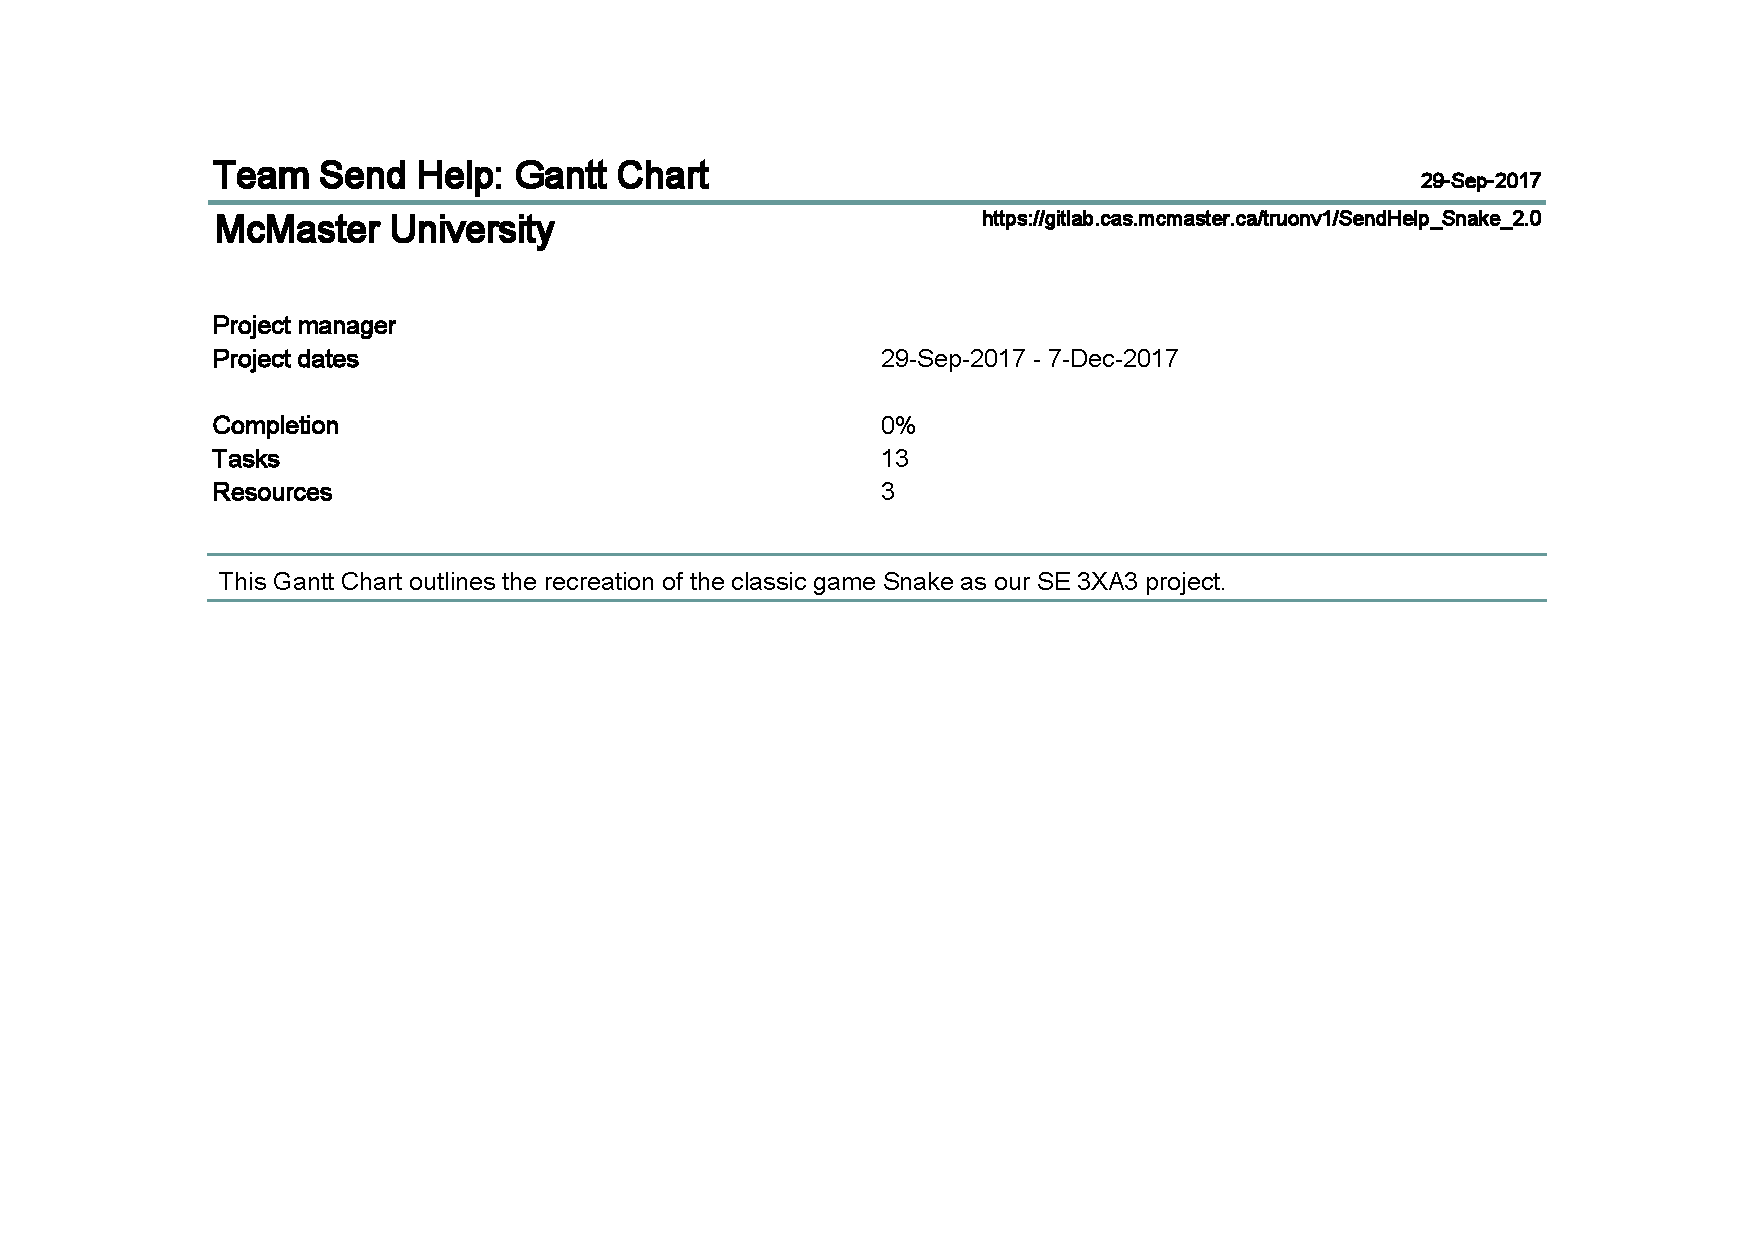
\includepdf[pages={-}]{GanttChart/SendHelp_GanttProject.pdf}

\end{document}
